\section{Wstęp}

\subsection{Opis problemu}

Głównym założeniem projektu było zapoznanie się biblioteką OpenMP na podstawie równoległego sumowania komórek tablicy. W ramach projektu zrealizowaliśmy 4 algorytmy sekwencyjne oraz 2 algorytmy zrównleglone. Celem zastosowania czterech różnych algorytmów sekwencyjnych było zbadanie wpływu sekcyjności pamięci podręcznej, wyprzdzającego pobrania danych do pamięcy podręcznej oraz kolejności uszeregowania pętli na czas realizacji zadania. W przypadku algorytmów zrównoleglonych badaliśmy wpływ kolejności uszeregowania pętli na końcowy rezultat.\newline

Nasze badania podzieliliśmy na 3 spójne części. Badaliśmy wpływ
\begin{itemize}
\item rozmiaru danych
\item sekcyjności pamięci
\item wyprzedzającego pobrania
\end{itemize}
na czas realizacji problemu.\newline

Sam problem sprowadzał się do zsumowania wartości komórek w tabeli. Dla zachowania czytelności w kolejności pętli zastosowaliśmy tablicę dwuwymiarową. Ponieważ sam problem jest prosty obliczeniowo zmuszeni byliśmy do stosowania bardzo dużych tablic typu int ($sizeof(int) = 4$), o rozmiarach 1GB ($[2^{24} - wierszy]$ na $[2^{4} - kolumn]$) i 256MB ($[2^{22} - wierszy]$ na $[2^{4} - kolumn]$).

W badanym systemie długość lini pamięci podręcznej wynosiła 64B, co odpowiada szerokości naszej tabeli. Aby zapewnić wyrównanie do początku lini PP tabela została zdefiniowana z wykorzystaniem rozszerzenia Visual Studio:

\begin{lstlisting}[caption=Definicja tabeli., captionpos=none]
__declspec(align(64)) int tab[ROWS][COLS];
\end{lstlisting}

\subsection{Punkt odniesienia (algorytm sekwencyjny -- kolejność ij)}

Punktem odniesienia dla wszystkich algorytmów był podstawowy algorytm sekwencyjny w którym sumowaliśmy elementy tablicy wierszami. Nazywany dalej $sum\_ij$.

\lstinputlisting[caption=Algorytm sekwencyjny -- kolejność ij.]{./code/sum_ij.cpp}


\subsection{Badane algorytmy}


\subsubsection{Algorytm sekwencyjny -- kolejność ji}

Algorytm sekwencyjny ze zmienioną kolejnością pętli (sumujemy kolumnami). Nazywany dalej $sum\_ji$.
\lstinputlisting[caption=Algorytm sekwencyjny -- kolejność ji]{./code/sum_ji.cpp}


\subsubsection{Algorytm zrównoleglony -- kolejność ij}

Algorytm sumujący wierszami realizowany równolegle. Nazywany dalej $sum\_par\_ij$.
\lstinputlisting[caption=Algorytm zrównoleglony -- kolejność ij.]{./code/sum_par_ij.cpp}


\subsubsection{Algorytm zrównoleglony -- kolejność ji}

Algorytm realizowany równolegle ze zmienioną kolejnością pętli (sumujemy kolumnami). Nazwywany dalej $sum\_par\_ji$.
\lstinputlisting[caption=Algorytm zrównoleglony -- kolejność ji.]{./code/sum_par_ji.cpp}


\subsubsection{Algorytm na sekcyjność pamięci}

Algorytm sekwencyjny w którym badaliśmy wpływ sekcyjności pamięci na czas wykonania zadania. Nazywany dalej $sum\_sec$.
\lstinputlisting[caption=Algorytm na sekcyjność pamięci.]{./code/sum_sec.cpp}


\subsubsection{Algorytm na pobranie z wyprzedzeniem}

Algorytm sekwencyjny w którym badaliśmy wpływ wyprzedzającego pobrania danych do pamięci podręcznej na czas realizacji zadania. Nazywany dalej $sum\_pf$.
\lstinputlisting[caption=Algorytm na pobranie z wyprzedzeniem.]{./code/sum_pf.cpp}

Ostatnia iteracja jest poza pętlą w celu uniknięcia konieczności sprawdzania czy nie został przekroczony zakres tablicy przy przypisaniu to $tmp$.

\subsection{Maska powinowactwa}

Aby wyeliminować przełączanie wykonywania wątku pomiędzy rdzeniami procesora zastosowaliśmy maski powinowactwa.

\subsubsection{Kod}

\lstinputlisting[caption=Ustawienie maski powinowactwa.]{./code/mask.cpp}

\subsubsection{Rezultat}

W rezultacie dla przetwarzania równoległego każdy wątek odpowiedzialny za sumowanie realizowany jest na oddzielnym procesorze. Co widoczne jest na poniższych wykresach:

\begin{figure}[Float]
\centering
\subfloat[sumowanie równoległe]{{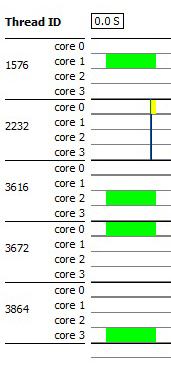
\includegraphics[width=0.4\textwidth]{mask_parallel.png} }}
\qquad
\subfloat[sumowanie sekwencyjne]{{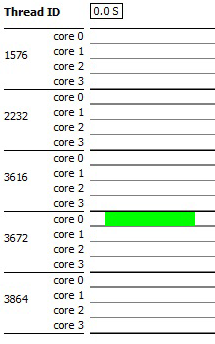
\includegraphics[width=0.4\textwidth]{mask_single.png} }}
\caption{Wykres przydziału wątków do rdzeni.}
\end{figure}
